\documentclass[12pt,a4paper]{article}
\usepackage{ctex}
\usepackage{amsmath,amscd,amsbsy,amssymb,latexsym,url,bm,amsthm}
\usepackage{epsfig,graphicx,subfigure}
\usepackage{enumitem,balance}
\usepackage{wrapfig}
\usepackage{mathrsfs, euscript}
\usepackage[usenames]{xcolor}
\usepackage{hyperref}
\usepackage[vlined,ruled,commentsnumbered,linesnumbered]{algorithm2e}
\usepackage{float}
\usepackage{array}
\usepackage{diagbox}
\usepackage{color}
\usepackage{indentfirst}
\usepackage{fancyhdr}
\usepackage{gensymb}
\usepackage{geometry}
\usepackage{setspace}
\usepackage{aurical}
\usepackage{times}
\usepackage{caption}
\usepackage{fontspec}
\usepackage{booktabs}
\usepackage{listings}
\usepackage{xcolor}
\setmainfont{Times New Roman}

\newtheorem{theorem}{Theorem}[section]
\newtheorem{lemma}[theorem]{Lemma}
\newtheorem{proposition}[theorem]{Proposition}
\newtheorem{corollary}[theorem]{Corollary}
\newtheorem{exercise}{Exercise}[section]
\newtheorem*{solution}{Solution}
\theoremstyle{definition}

\newcommand{\tabincell}[2]{\begin{tabular}{@{}#1@{}}#2\end{tabular}}
\newcommand{\postscript}[2]
 {\setlength{\epsfxsize}{#2\hsize}
  \centerline{\epsfbox{#1}}}

\renewcommand{\baselinestretch}{1.05}

\setlength{\oddsidemargin}{-0.365in}
\setlength{\evensidemargin}{-0.365in}
\setlength{\topmargin}{-0.3in}
\setlength{\headheight}{0in}
\setlength{\headsep}{0in}
\setlength{\textheight}{10.1in}
\setlength{\textwidth}{7in}
\makeatletter \renewenvironment{proof}[1][Proof] {\par\pushQED{\qed}\normalfont\topsep6\p@\@plus6\p@\relax\trivlist\item[\hskip\labelsep\bfseries#1\@addpunct{.}]\ignorespaces}{\popQED\endtrivlist\@endpefalse} \makeatother
\makeatletter
\renewenvironment{solution}[1][Solution] {\par\pushQED{\qed}\normalfont\topsep6\p@\@plus6\p@\relax\trivlist\item[\hskip\labelsep\bfseries#1\@addpunct{.}]\ignorespaces}{\popQED\endtrivlist\@endpefalse} \makeatother

\begin{document}
\noindent
%==========================================================
\noindent\framebox[\linewidth]{\shortstack[c]{
\Large{\emph{模型评价与模型改善}}\vspace{1mm}\\
CS245 \quad 数据科学基础 \quad 陆朝俊 \vspace{1mm} \\
叶泽林 515030910468}}

\section{问题描述}

给定一个机器学习问题(如分类)以及相应的数据集,可以训练出一个初步的模型,但在投入实际应用前,需要对该模型的性能进行评价甚至改善。一般地,通过组合模型的方式,可以提高模型的效果。这次作业中,我将在自己建立的分类数据集上探索决策树模型单独工作以及组合工作时的性能。

\section{解决方案\protect\footnote{本次作业的所有代码实现可参见附录 \ref{apd:code}}}

\subsection{数据集的建立及模型的选择}

由于现有的中小型数据集存在一些难以满足实验要求的属性,我选择自己建立一个分类数据集$D$(后文均以$D$表示此数据集),之后的所有实验均基于此数据集上进行。数据集$D$包含500个样本,30个特征(存在冗余和重复的特征),为更好地看出模型性能的区别,我在$D$中添加了部分噪声。关于数据集$D$详细的设定参数可参考附录 \ref{apd:dataset_para}。

解决分类问题的机器学习模型主要有逻辑回归、决策树以及KNN,在这次作业中,我选择决策树作为探索的模型。

\subsection{探索模型单独工作的性能}

选定数据集和模型后,我首先探索单独的决策树模型在数据集$D$上的性能,探索方法如下:

\begin{enumerate}
\item \textbf{直接划分训练集和测试集}

在一般应用中,对模型性能最朴素的评价方法即为:将数据集划分为训练集和测试集,在训练集上训练模型后,根据模型在测试集上的表现评价模型性能。因此,我首先采用这个方法对模型的性能进行一个粗略的估计。

\item \textbf{分层交叉验证}

从理论上说,仅凭在一个训练集$D_1$上训练出的模型$M_1$无法代表模型$M$(在我的实验中为决策树模型)解决这个问题的效果。分层交叉验证正好解决了这一问题,其步骤大致如下:

\begin{enumerate}
	\item 将数据随机等分为$k$个不相交子集$D_1, D_2, ... ,D_k$(每个子集的类分布与初始数据近似相同);
	
	\item 总共执行$k$次训练与测试,在第$i$折时,使用$D_i$作为测试集, 其他子集作为训练集;
	
	\item 模型的性能由$k$次迭代的平均效果决定。
\end{enumerate}

分层交叉验证相当于在同一个数据集上进行了多次训练集-测试集划分。和简单的训练集-测试集划分相比,能更准确地评估模型来自样本的误差。

\item \textbf{网格搜索}

网格搜索是通过蛮力试验不同参数组合,从而选择最佳模型的方法。理论上来说,网格搜索与分层交叉验证相结合,可以找出模型解决给定问题最合适的参数,但这一过程需要花费大量的时间和计算资源,因此这次作业中我仅实现了一小部分参数空间上的网格搜索。

\end{enumerate}

\subsection{探索模型组合工作的性能}

一般地,从一系列模型$M_1, M_2, ... , M_k$创建组合模型$M^*$,可以有效提高原模型的效果。组合方法主要分为bagging和boosting两种。Bagging方法使用并行思想,$M^*$通过整合各原模型的结果得到输出;Boosting方法则采用串行思想,利用模型$M_{i-1}$的训练结果训练模型$M_{i}$,直到$M_k$。

\section{结果展示}

\subsection{模型单独工作的性能}
\label{sec:pca_res_com}

\subsubsection{直接划分训练集和测试集}

首先,我将原数据按照一定比例划分为训练集和测试集,划分时保证每一类型的数据在训练集和测试集的占比大致服从原分布,再执行一般的“训练集上训练-测试集上测试”流程。测试结果如表 \ref{tab:train-test} 所示。

\begin{table}[H]
	\renewcommand\arraystretch{1.35}
	\caption{训练集-测试集划分探索模型在$D$上的性能}
	\label{tab:train-test}
	\centering
	
	\begin{tabular}{c|c|c|c|c}
		\centering
		\tabincell{c}{测试集占比(其中\\0表示随机分类)} & \tabincell{c}{测试集上平均\\精确度} & \tabincell{c}{测试集上平均\\召回率} & \tabincell{c}{测试集上平均\\f1-score} & \tabincell{c}{训练集上平均\\f1-score} \\
		\hline
		0 & 0.59 & 0.56 & 0.56 & 1.00 \\
		0.05 & 0.78 & 0.72 & 0.73 & 1.00 \\
		0.1 & 0.59 & 0.56 & 0.56 & 1.00 \\
		0.2 & 0.57 & 0.56 & 0.56 & 1.00 \\	
		0.3 & 0.57 & 0.56 & 0.56 & 1.00 \\	
		0.4 & 0.56 & 0.56 & 0.55 & 1.00 \\
		0.5 & 0.50 & 0.48 & 0.48 & 1.00 \\
		0.8 & 0.49 & 0.48 & 0.48 & 1.00 \\
	\end{tabular}
\end{table}

粗略测试的结果表明:不论训练集-测试集的划分比例如何,该模型总是趋于过拟合,对新数据的分类效果较差。

\subsubsection{分层交叉验证}

上小节仅对决策树模型在$D$上单独工作的性能进行了粗略的估计,下面使用分层交叉验证对模型单独工作的性能做更完整的探索,结果参见图 \ref{fig:cv_bar}。

\begin{figure}[H]
	\centering
	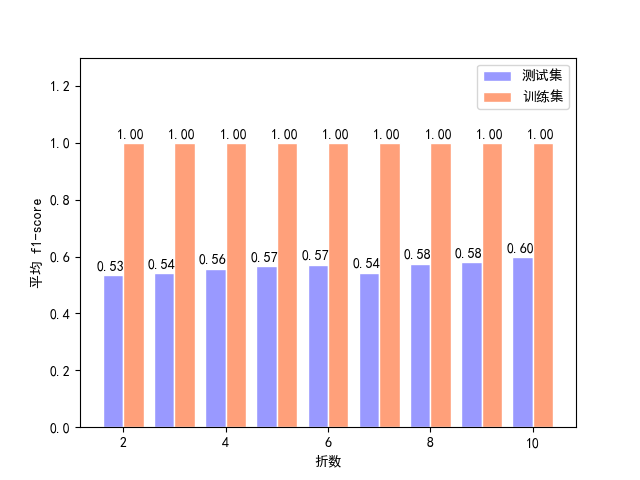
\includegraphics[width=0.8\linewidth]{img/cv_bar.png}
	\caption{分层交叉验证探索模型在$D$上的性能}
	\label{fig:cv_bar}
\end{figure}

从图中可以看出,折数和在测试集上的f1-score呈正相关(折数越多,训练集则越大,模型对$D$学习得更充分),但均在0.5与0.6之间,对于一般应用来说也属于较低水平。除此之外,在训练集上的高f1-score也说明模型的过拟合问题尤为严重。

\subsubsection{网格搜索}

这部分实验中,我结合网格搜索和分层交叉验证(10折),得到决策树模型在$D$上的最佳效果。由于遍历所有参数需要消耗大量的时间和计算资源,我在实验中仅选择了模型的部分重要参数进行网格搜索。具体结果可参见表 \ref{tab:grid-search}。

\begin{table}[H]
	\renewcommand\arraystretch{1.35}
	\caption{网格搜索结果}
	\label{tab:grid-search}
	\centering
	
	\begin{tabular}{c|c|c|c}
		\centering
		参数名 & 参数含义 & 参数范围 & 模型效果最佳时的值 \\
		\hline
		criterion & 特征选择的度量标准 & gini, entropy & gini \\
		\hline
		max\_depth & 树的最大深度 & 正整数 & 9 \\
		\hline
		max\_features & \tabincell{c}{寻求最佳划分时\\要考虑的特征数目} & \tabincell{c}{总特征数或其平方根\\或其以2为底的对数值} & 总特征数 \\
		\hline
		presort & 是否对数据预先排序 & True, False & True \\
		\hline
		splitter & 结点划分策略 & best, random & best \\
	\end{tabular}
\end{table}

经过对上表参数值的网格搜索,得到的模型在分层交叉验证中各测试集的平均f1-score为0.61,虽然只遍历了一部分参数空间,但这个结果在一定程度上也能够代表决策树模型在$D$上分类的最佳性能。最佳模型的可视化结果可参见附录 \ref{apd:vis-tree}。

\subsubsection{结果分析}

通过上面三个小节的探索,可以得出结论:决策树模型单独工作时,在数据集$D$上分类的f1-score基本在0.5-0.6之间,最高仅达0.61,而在训练集上的分类效果极佳,表明该模型在$D$上单独工作时容易趋于过拟合,对新数据的分类效果较差。

\subsection{模型组合工作的性能}

\subsubsection{bagging}

\subsubsection{boosting}

\subsubsection{结果分析}

\section{结论}

\newpage
\begin{appendix}
	\section{附录}
	\subsection{分类数据集$D$的详细信息}
	\label{apd:dataset_para}
	\begin{table}[H]
		\renewcommand\arraystretch{1.35}
		\caption{分类数据集$D$的详细信息}
		\label{tab:dataset_para}
		\centering
		
		\begin{tabular}{c|c}
			\centering
			属性 & 值 \\
			\hline
			样本个数 & 50 \\
			特征个数 & 30 \\
			类个数 & 3 \\
			类分布 & 每个类均匀分布 \\
			包含信息的特征占比 & 0.6 \\
			冗余特征的占比(含信息特征的线性组合) & 0.1 \\
			重复特征的占比(随机取自含信息特征和冗余特征) & 0.1 \\
			噪声占比 & 0.03 \\		
		\end{tabular}
	\end{table}
	
	\subsection{决策树单独工作的最佳模型可视化}
	由于图片较大,若有需要可放大后详细观看,不影响图片清晰度。
	\label{apd:vis-tree}
	\begin{figure}[H]
		\centering
		
\includegraphics[width=0.9\linewidth]{img/gs.pdf}
		\caption{决策树单独工作的最佳模型}
	\end{figure}
	
	\subsection{主要代码}
	\label{apd:code}
	
	\begin{lstlisting}[language=Python,
	numbers=left,
	keywordstyle=\color{blue!70},
	frame=shadowbox,
	breaklines=True]
import matplotlib.pyplot as plt
plt.rcParams['font.sans-serif'] = ['SimHei']    # display Chinese
plt.rcParams['axes.unicode_minus'] = False      # display minus sign
from mpl_toolkits.mplot3d import Axes3D
from sklearn import datasets
from sklearn.decomposition import PCA

import os
import time

class bostonAnalyzer(object):
    def __init__(self):
        # load dataset
        self.dataset = datasets.load_boston()
        self.data = self.dataset.data
        self.target = self.dataset.target
        
        # for plot
        self.var = []
        self.t = []

        if not os.path.exists('report/img'):
            os.makedirs('report/img')

    def run(self, vis=False):
        '''
        Run PCA for 1-13 dimensions
        :param vis: True: plot dim 1-3; False: not plot
        '''

        self.var.clear()
        self.t.clear()

        with open('report/result.txt', 'w') as f:
            for i in range(13):
                t = time.time()
                pca_op = PCA(n_components=i)
                pca_res = pca_op.fit_transform(self.data)
                t = time.time() - t

                self.var.append(pca_op.explained_variance_ratio_.sum())
                self.t.append(t)

                # write log
                f.write('###### Dimension %d ######\n' % i)
                f.write(str(pca_res.shape) + '\n')
                f.write(str(pca_op.explained_variance_ratio_) + '\n')
                f.write(str(pca_op.explained_variance_ratio_.sum()) + '\n')
                f.write(str(t) + '\n\n')

                # visualize for debug & plot
                if vis:
                    if i == 1:
                        # plot 1 dimension
                        plt.scatter(pca_res[:, 0], pca_res[:, 0], s=14, c=self.target)
                        plt.savefig('report/img/pca-%d' % i)
                        plt.show()
                    elif i == 2:
                        # plot 2 dimensions
                        plt.scatter(pca_res[:,0], pca_res[:,1], s=8, c=self.target)
                        plt.savefig('report/img/pca-%d' % i)
                        plt.show()
                    elif i == 3:
                        # plot 3 dimensions
                        ax = plt.subplot(projection='3d')
                        ax.scatter(pca_res[:, 0], pca_res[:, 1], pca_res[:, 2], s=8, c=self.target)
                        plt.savefig('report/img/pca-%d' % i)
                        plt.show()

    def show(self):
        '''
        Show the basic info of Boston dataset & plot k-lines
        '''
        print(self.data.shape)
        print(self.target.shape)
        self._k_line_radio()
        self._k_line_time()

    def _k_line_radio(self):
        '''
        Plot k-line of variant radio
        '''
        x = list(range(len(self.var)))
        plt.scatter(x, self.var, s=14, c='r')
        plt.plot(x, self.var)
        plt.xlabel('主成分个数')
        plt.ylabel('降维后各特征方差比例之和')
        plt.savefig('report/img/kline-radio')
        plt.show()

    def _k_line_time(self):
        '''
        Plot k-line of time
        '''
        x = list(range(len(self.t)))
        plt.scatter(x, self.t, s=14, c='r')
        plt.plot(x, self.t)
        plt.xlabel('主成分个数')
        plt.ylabel('PCA算法消耗时间(s)')
        plt.savefig('report/img/kline-time')
        plt.show()

if __name__ == '__main__':
    bA = bostonAnalyzer()
    bA.run(True)
    bA.show()
	\end{lstlisting}
	
\end{appendix}

%========================================================================
\end{document}